\documentclass[a4paper]{extarticle}
\usepackage[utf8]{inputenc}
\usepackage[a4paper, margin=1in]{geometry}

\usepackage{amssymb}
\usepackage{amsmath}
\usepackage{enumitem}
\usepackage{tcolorbox}
\usepackage{fancyhdr}
\usepackage{graphicx}
\usepackage{float}

\setlength{\parindent}{0em}
\setlength{\parskip}{0.4em}

\definecolor{theoremblue}{RGB}{1, 73, 124}
\definecolor{corollaryblue}{RGB}{70, 143, 175}
\definecolor{exampleblue}{RGB}{137, 194, 217}

\newtcolorbox{tbox}{colback=theoremblue!20,colframe=theoremblue,
boxrule=0pt,arc=0pt,boxsep=2pt,left=2pt,right=2pt,leftrule=2pt}

\newtcolorbox{cbox}{colback=corollaryblue!20,colframe=corollaryblue,
boxrule=0pt,arc=0pt,boxsep=2pt,left=2pt,right=2pt,leftrule=2pt}

\newtcolorbox{ebox}{colback=exampleblue!20,colframe=exampleblue,
boxrule=0pt,arc=0pt,boxsep=2pt,left=2pt,right=2pt,leftrule=2pt}

\title{IntroML - Lecture Notes Week 6}
\author{Ruben Schenk, ruben.schenk@inf.ethz.ch}
\date{\today}

\pagestyle{fancy}
\fancyhf{}
\rhead{ruben.schenk@inf.ethz.ch}
\rfoot{Page \thepage}
\lhead{IntroML - Lecture Notes Week 6}

\begin{document}

\maketitle

\section{Neural Networks}

\subsection{Features}

The success in learning crucially depends on the quality of \textbf{features.} But what about kernel methods? Don't they yield "universal" features?
\begin{itemize}
    \item They provide a set of rich feature maps: can approximate "any function" given infinite data
    \item Give finite data, the choice of the kernel matters a lot!
    \item Choosing the "right" kernel can be challenging
\end{itemize}

\subsection{Learning Features}

Can we \textbf{learn} good features from data directly? Consider learning with $m$ hand-designed features:

\[
    w^* = \arg \min_w \sum_{i = 1}^n l \Big (y_i; \, \sum_{j = 1}^m w_j \phi_j(x_i)\Big )
\]

The key idea is to parameterize the feature maps, and optimize over the parameters:

\[
    w^* = \arg \min_{w, \, \theta_j} \sum_{i = 1}^n l \Big ( y_i; \, \sum_{j = 1}^m w_j \phi(x_i; \, \theta_j) \Big)
\]

But how do we parameterize feature maps? The design idea is as follows. We build \textit{complex models} out of simple components, for example:

\[
    \phi(x, \, \theta) = \rho (\theta^Tx),
\]

where $\theta \in \mathbb{R}^d$ and $\rho : \mathbb{R} \to \mathbb{R}$ is a non-linear (simple) \textit{activation function.}

\begin{ebox}
    \textbf{Examples:} Following some simple activation functions:
    \begin{itemize}
        \item Identity: $\rho(z) = z$
        \item Sigmoid: $\rho(z) = \frac{1}{1 + \exp(-z)}$
        \item Tanh: $\rho(z) = \tanh(z)$
        \item Rectified linear unit (ReLU): $\rho(z) = \max(0, \, z)$
    \end{itemize}
\end{ebox}

\subsection{Artificial Neural Networks (ANNs)}

Nested functions of the form

\[
    f(x; \, w, \, \theta) = \sum_{j = 1}^m w_j \rho (\theta_j^T x)
\]

are examples of \textbf{artificial neural networks (ANNs),} also called \textit{multi-layer perceptrons.} More generally, the term artificial neural network refers to non-linear functions which are nested compositions of (learnable) linear functions composed with (fixed) non-linearities.

\begin{figure}[H]
    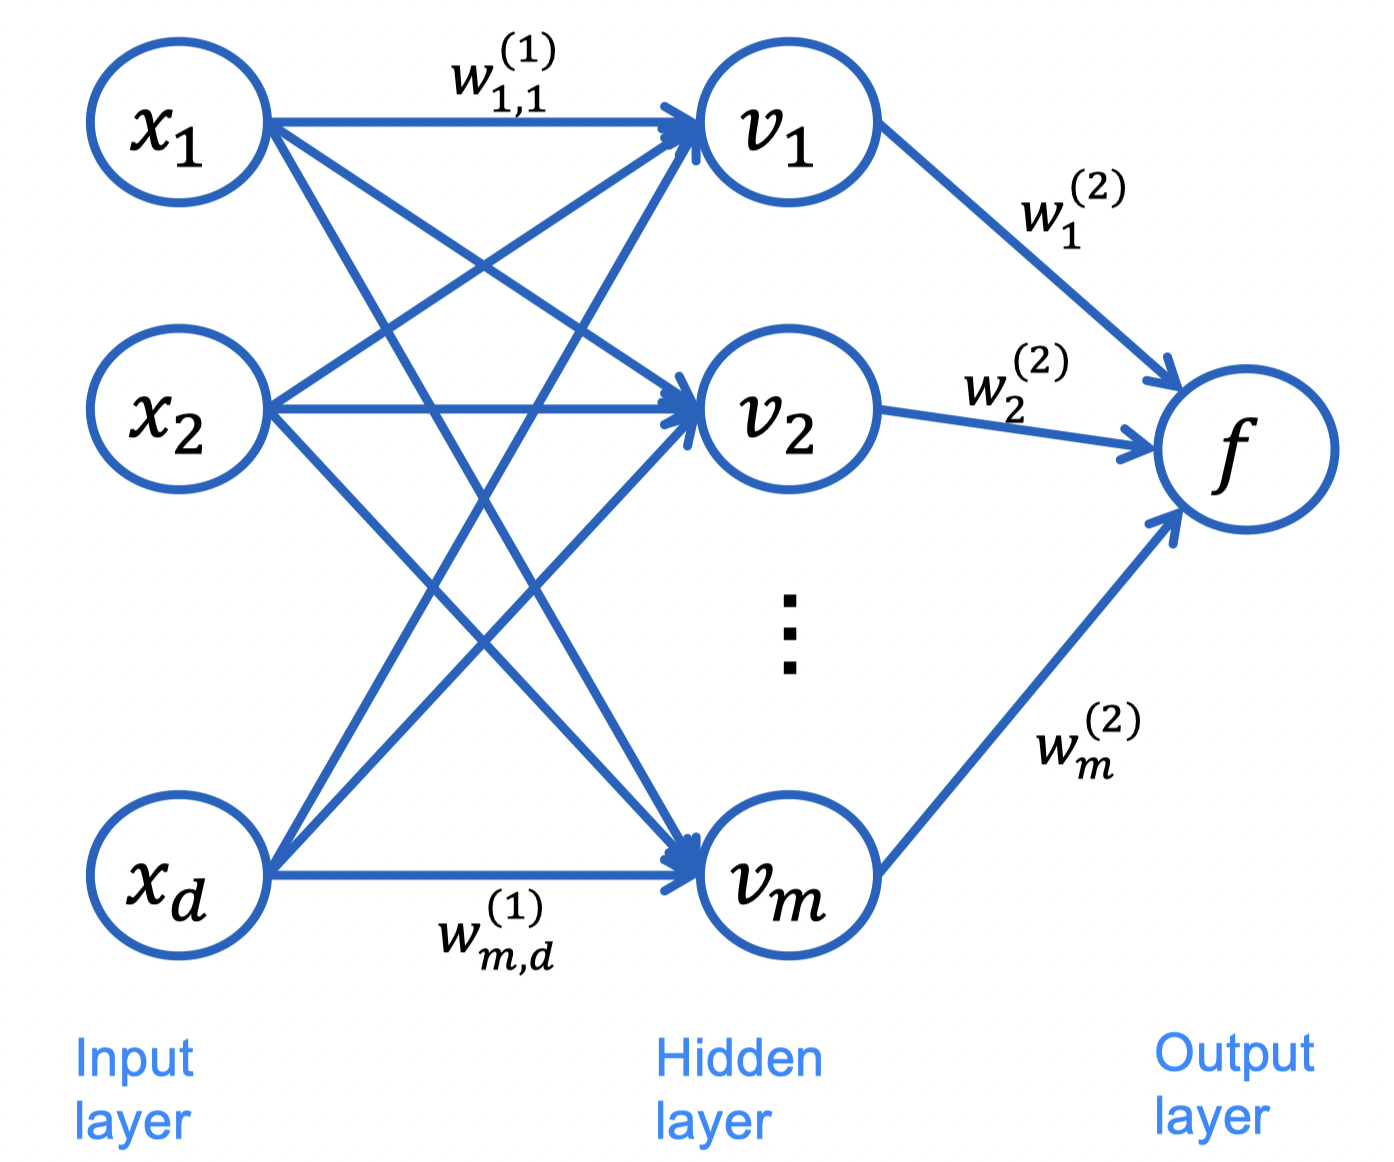
\includegraphics[width=8cm]{../images/IntroML_Fig6-1}
    \centering
\end{figure}

We can deal with biases by introducing a "constant $1$" feature not only to the inputs, but also to the hidden layers. These "constant $1$" units have no incoming connections/weights.

\subsection{Universal Approximation Theorem}

\begin{tbox}
    \textbf{Theorem:} Let $f$ be any continuous function on $[0, \, 1]^d$ and $\rho$ any sigmoidal activation function. Then $f$ can be uniformly approximated by a finite sum of the form:

    \[
        \hat{f}(x) = \sum_{j = 1}^m w_j^{(2)}\rho(w_j^{(1)T}x + w_{j,0}^{(1)})
    \]
\end{tbox}

\end{document}